\chapter{AreaComp}

\section{Konzept}

Sei $S = s_0, \dots, s_{n-1} \in \Sigma^*$ mit $n := |S|$ ein String über ein Alphabet $\Sigma$.

Ein Intervall $LCP[i..j]$ mit $0 \leq i \leq j < n$ im LCP-Array beschreibt wiederholte Vorkommen von Substrings. Aus diesem Intervall lässt sich schließen, wie oft dieser Substring vorkommt, wie lang dieser ist, und mithilfe des Suffix-Arrays lässt sich feststellen, wo dieser vorkommt. Jeder Eintrag $LCP[k], k = 1,\dots,n-1$ im LCP-Array ist die Länge des längsten gemeinsamen Präfixes der beiden Suffixe ist, die bei $SA[k-1]$ und $SA[k]$ beginnen. Daher gilt dann folgendes:

An den Indizes $I = \{SA[i]\ |\ i \in \{i-1, \dots, j\}\}$ befindet sich jeweils ein Vorkommen eines Substrings der Länge $l = \min_{k = i, \dots, j} LCP[k]$. Wir nennen dann $W(i, j) := |I| = j - i + 2$ die Breite von $LCP[i..j]$ und $H(i, j) := l$ die Höhe von $LCP[i..j]$.\\\\
Intervalle mit großer Breite (viele Vorkommen) bzw. Höhe (langer Substring) bieten also eine besonders große Kompression, wenn diese Vorkommen durch ein Nichtterminal und eine entsprechende Produktionsregel ersetzt werden.

Es ist hier also eine Art Gütefunktion $A: \mathbb{N}_0 \times \mathbb{N}_0 \rightarrow \mathbb{N}_0$ nötig, die Intervalle je nach potentieller Kompression bewertet. Diese Funktion nennen wir Flächenfunktion. Je größer der von der Funktion gelieferte Wert, desto nützlicher ist das Intervall.\\\\
Die Idee ist also, inkrementell eine Straight Line Grammatik zu erzeugen. Dies geschieht durch die wiederholte Wahl eines vielversprechenden Intervall im LCP-Array anhand der Flächenfunktion. Jedes Vorkommen des von dem Intervall bestimmten Substring wird durch ein neues Nichtterminal und eine entsprechende neue Produktionsregel der Grammatik ersetzt.\\

Dies wird solange wiederholt bis keine Intervalle mehr übrig sind, die einen nützlichen Wert der Flächefunktion liefern. Etwa müssen Intervalle der Fläche $0$, bei der oben vorgeschlagenen Flächenfunktion nicht betrachtet werden.\\

Die Priorisierung von Intervallen anhand der Flächenfunktion kann mithilfe einer Prioritätswarteschlange umgesetzt werden. Die Intervalle werden mit dem Gewicht $A(i, j)$ eingefügt. So kann in jedem Durchlauf ein Element in der richtigen Reihenfolge entnommen werden.\\\\

\subsection{Beispiel}

Zunächst ein Beispiel für einen Durchlauf: Wir wählen die Flächenfunktion
\begin{equation}
	A[i, j] := \min \{ lcp[x]\ |\ i \leq x \leq j\} \cdot (j - i)
\end{equation} 
und betrachten den String $S =$ \enquote{ababcaba\$}. Dann gilt:

\begin{figure}[H]
	\centering
	\begin{tabular}{|c|c|c|l|} \hline
		$i$ & $SA$ & $LCP$ & Suffix\\ \hline
		$0$ & $8$ & $0$ & \$ \\\hline
		$1$ & $7$ & $0$ & a\$ \\\hline
		$2$ & $5$ & $1$ & aba\$ \\\hline
		$3$ & $0$ & $3$ & ababcaba\$ \\\hline
		$4$ & $2$ & $2$ & abcaba\$ \\\hline
		$5$ & $6$ & $0$ & ba\$ \\\hline
		$6$ & $1$ & $2$ & babcaba\$ \\\hline
		$7$ & $3$ & $1$ & bcaba\$ \\\hline
		$7$ & $4$ & $0$ & caba\$ \\\hline
	\end{tabular}
\end{figure}

Wir beginnen mit der leeren Grammatik $S \rightarrow ababcaba\$$. Die Intervalle mit maximalem $A$ sind $LCP[2..3]$ und $LCP[3..3]$. $A(2, 3) = A(3, 3) = 6$.\\
Wählt man nun das Intervall $LCP[3..4]$ so gilt entsprechend $W(3, 4) = 3$ und $H(3, 4) = 2$. Der zu ersetzende Substring ($ab$) ist also zwei Zeichen lang und kommt dreimal im String vor.\\
Wir erzeugen nun eine neue Produktionsregel $A \rightarrow ab$ und ersetzen jedes Vorkommen von $ab$ in der Grammatik durch $A$.
Die resultierende Grammatik ist dann also:
\begin{align*}
	S &\rightarrow AAcAa\\
	A &\rightarrow ab
\end{align*}

Es gibt nun keine wiederholten Zeichenfolgen mehr und der Algorithmus terminiert.

\subsection{Überlegungen}

\subsubsection{Überlappungen}

Es kann vorkommen, dass ein zu ersetzendes Muster überlappend vorkommt, wie etwa $aa$ im String $aaa$. In diesem Fall können die überlappenden Vorkommen nicht ersetzt werden. Hier muss also Acht gegeben werden. Gegebenfalls müssen also alle Positionen ignoriert werden, die sich überlappen.

\subsubsection{Überschneidende Substitutionen}

Es können aber auch in einem Schritt eine Substitution durch ein LCP-Intervall $I_1 := LCP[i_1..j_1]$ durchgeführt worden sein, die sich mit einer späteren Substitution durch ein LCP-Intervall $I_2 := LCP[i_2..j_2]$ überschneiden. In diesem Fall, kann der tatsächliche Nutzen der Substitution sinken. Es muss also dafür gesorgt werden, dass bereits ersetzte Teile des Strings nicht nochmals ersetzt werden.

\newpage
\section{AreaComp V1}

Die erste Version ist eine naive Implementierung. Der Algorithmus verwaltet eine Menge von Regeln. Jede Regel besitzt eine einzigartige natürliche Zahl als ID. Der Begriff \emph{Regel} wird synonym mit dessen Regel-ID verwendet. 

In jedem Durchlauf wird nacheinander jede Regel $(X \rightarrow w) \in P$ aus der Menge entnommen und das Suffix- und LCP-Array für die rechte Seite dieser Regel berechnet. Es wird nun eine Prioritätswarteschlange erzeugt, die alle möglichen LCP-Intervalle enthält. Das beste LCP-Intervall nach Flächenfunktion wird daraus entnommen. Sei $p \in (N \cup \Sigma)^*$ das, durch das LCP-Intervall bestimmte, zu ersetzende Muster. Die Indizes, an denen ein Vorkommen von $p$ in $w$ existiert, kann einfach mithilfe des Suffix- und LCP-Array berechnet werden.

Es werden nun alle bestimmten Vorkommen darauf untersucht, ob sich diese mit Anderen überschneiden. Hierzu werden die Indizes, an denen $p$ vorkommt, aufsteigend sortiert und durchlaufen. Dabei werden alle Indizes gelöscht, die einen Abstand von weniger als $|p|$ zum letzten Index haben. Damit bleiben nur Vorkommen übrig, die sich nicht überschneiden. Sind nun nur noch weniger als zwei Positionen übrig, so wird das nächst-beste LCP-Intervall aus der Warteschlange entnommen und der Vorgang wiederholt. Sind keine Intervalle mehr übrig, so fahre zur nächsten Produktionsregel fort.

Der von diesem Intervall bestimmte Substring wird dann durch ein neues Nichtterminal und eine zugehörige Produktionsregel ersetzt. Zu diesem Zweck wird die gesamte Grammatik nach Vorkommen durchsucht und diese durch das Nichtterminal ersetzt.

Die Datenstruktur, mit der Regeln, Terminale und Nichtterminale verwaltet werden, ist gleich der Datenstruktur, die Sequitur benutzt. Allerdings verwendet der Algorithmus zusätzlich eine Hashtabelle, die eine Regel-ID auf das zugehörige Regel-Objekt abbildet.

Diese Implementierung hat nicht das Problem, dass sich Substitutionen entstehen können, die sich mit vorherigen Substitutionen überschneiden, da Suffix- und LCP-Array für jede einzelne Regel in jedem Durchlauf neu erzeugt werden. 

\begin{algorithm}[t]
    \KwIn{$s:$ String}
    \KwOut{Straight-Line-Grammatik für $s$}
    \While{ Eine neue Regel kann erzeugt werden }{
        \For{Regel \texttt{rule} in der Regelmenge}{
            $SA, LCP \leftarrow$ Suffix- und LCP-Array für rechte Seite von $rule$\;
            $queue \leftarrow$ Prioritätswarteschlange aller LCP-Intervalle der rechten Seite von $rule$, geordnet mithilfe der Flächenfunktion\;
            \Do{$queue \neq \emptyset$ \And $positions.length \leq 1$}{
                $[l..r] \leftarrow queue.poll()$\;
                $positions \leftarrow$ Array der Indizes der Vorkommen des durch $[l..r]$ beschriebenen Musters (mithilfe von $SA$)\;
                $len \leftarrow \min_{i \in [l..r]} LCP[i]$\;
                Sortiere $positions$ aufsteigend\;
                Entferne überlappende Vorkommen aus $positions$\;
            }
            \If{$positions.length \leq 1$}{
                \KwBreak \;
            }
            Substituiere alle Vorkommen in $positions$ mit der Länge $len$\;
        }
    }
    \KwRet{Regelmenge}
    \caption{AreaCompV1}
    \label{v1algo}
\end{algorithm}

\subsection{Probleme}

\subsubsection{Laufzeit}
\label{v1problemruntime}

Das größte Problem dieser Implementierung ist die Laufzeit. Sei $s \in \Sigma^*$ mit $n := |s|$ der Eingabestring.

Wie in \autoref{v1algo} dargestellt, wird in jedem Durchlauf der While-Schleife jeweils durch die Menge der zu diesem Zeitpunkt existierenden Regeln iteriert. 
In jedem Durchlauf wird für jede Regel $rule := X \rightarrow w \in P, X \in N, w \in (N \cup \Sigma)^*$ das in Bezug auf die Flächenfunktion beste LCP-Intervall im LCP-Array von $w$ berechnet. Dessen Berechnung dominiert die Laufzeit dieser Version des Algorithmus. 
Es existieren $|w|^2$ solche Intervalle. Für jedes dieser LCP-Intervalle muss die Flächenfunktion berechnet werden, da diese in die Prioritätswarteschlange eingefügt werden müssen (Zeile 4). Eine Flächenfunktion, die alle Werte in ihrem gegebenen LCP-Intervall $I$ in Betracht zieht, muss mindestens eine Laufzeit von $\mathcal{O}(|I|)$ haben, da das Minimum im Intervall linear gesucht werden muss.

Im Worst-Case kann in $w$ keine Substitution mehr durchgeführt werden kann. In diesem Fall muss die Do-While-Schleife alle $|w|^2$ Intervalle verarbeiten. Jeder Durchlauf der Do-While-Schleife benötigt $\mathcal{O}(|w| \log |w|)$ Laufzeit, dominiert durch das Sortieren des $positions$ Array. Also folgt eine Worst-Case Laufzeit von $\mathcal{O}(|w|^3 \log |w|)$ für einen Durchlauf der For-Schleife. Die For-Schleife wird pro Durchlauf der While-Schleife für jede Regel in der Regelmenge einmal durchlaufen. Da $|w|$ in $\mathcal{O}(n)$ liegt, resultiert eine Laufzeit von $\mathcal{O}(n^3 \log n)$ für einen Durchlauf der For-Schleife.

Die Anzahl an Regeln ist durch $\mathcal{O}(n)$ Regeln beschränkt, denn ist die Anzahl von Regeln größer als linear, so kann keine Kompression stattfinden. Also folgen $\mathcal{O}(n)$ Durchläufe der For-Schleife pro Durchlauf der While-Schleife und damit insgesamt $\mathcal{O}(n^4 \log n)$ Laufzeit.

Da die Gesamtlänge der Grammatik $n$ nicht überschreiten kann und die Größe der Grammatik in jedem Durchlauf der While-Schleife um mindestens $1$ sinken muss, können im Worst-Case $\mathcal{O}(n)$ Iterationen der While-Schleife stattfinden. Insgesamt folgt im Worst-Case also eine Laufzeit von $\mathcal{O}(n^5 \log n)$.


\subsubsection{Erkennung von Wiederholungen}

Diese Version des Algorithmus erkennt keine wiederholten Vorkommen von Substrings, falls diese in verschiedenen Produktionsregeln auftreten.
Etwa würde in der folgenden Grammatik das wiederholte Vorkommen von $abc$ nicht erkannt werden:

\begin{align*}
	S &\rightarrow AA\textcolor{red}{abc}\\
	A &\rightarrow cdef\textcolor{red}{abc}
\end{align*}

Dies liegt daran, dass das Suffix- und LCP-Array, in dem nach wiederholten Vorkommen gesucht wird, für jede Produktionsregel einzeln berechnet werden. Dabei werden natürlich alle Vorkommen außerhalb dieser Produktionsregel nicht erfasst.
\newpage
\section{AreaComp V2}


Gegenüber der ersten Version des Algorithmus gibt es mehrere Verbesserungen:

\subsection{Datenstrukturen} Regeln bestehen nun nicht mehr aus der verketteten Struktur wie bei Sequitur. Stattdessen besitzt eine Produktionsregel nun zwei dynamische Arrays. \texttt{symbols} enthält die Symbole und \texttt{cumulativeLength} ist die Präfixsumme über die (voll expandierte) Länge der einzelnen Symbole in der Symbolliste.

Sei zum Beispiel die Grammatik: 
\begin{align*}
	A &\rightarrow BBde\\
	B &\rightarrow abc
\end{align*}
Dann gilt für die Produktionsregel $A$: 
\begin{align*}
	\texttt{symbols} &= [B, B, d, e]\\
	\texttt{cumulativeLength} &= [3, 6, 7, 8]
\end{align*}

\subsection{Suffix- und LCP-Array}
Im Gegensatz zu Version 1 wird in Version 2 das Suffix- und LCP-Array, und damit auch die Prioritätswarteschlange, nur einmal zu Anfang des Algorithmus global für den Eingabestring berechnet. Damit ist die wiederholte Berechnung in jedem Durchlauf nicht mehr nötig. 
Dadurch wird ebenfalls das Problem behoben, dass V1 wiederholte Vorkommen eines Musters nicht erfasst, die nicht in derselben Regel liegen.

Dies hat allerdings auch Auswirkungen auf den Algorithmus, die neue Probleme schaffen. Im Gegensatz zu den in V1 berechneten Suffix- und LCP-Arrays, ändern sich Suffix- und LCP-Array in V2 nicht, wenn Substitutionen stattfinden. 

Sei $s = s_0, \dots, s_{n-1} \in \Sigma^*$ mit $n := |s|$ der Eingabestring und $p \in \Sigma^*$ mit $\ell := |p|$  ein zu substituierendes Muster und $id_p \in \mathbb{N}$ die Regel, die auf $p$ abbildet. Zusätzlich sei $i \in \mathbb{N}, 0 \leq i \leq n - \ell$ ein Index in $s$. Wird nun ein Vorkommen von $p$ in $s$ bei Index $i$ ersetzt, so heißt das Intervall $[i.. i + \ell - 1]$ \emph{Ersetzungsintervall} der Regel $id_p$ bei Index $i$. Dabei wird das Intervall $[0, n-1]$ zu Beginn des Algorithmus als Ersetzungsintervall der Regel $R_0$ erzeugt, wobei $R_0$ die Startregel ist.

\subsection{Neue Datenstrukturen}

\begin{figure}
	\centering
	
    \subfloat[Eine Grammatik für den String $abcdbcabcde$.]{
        \makebox[8cm] {
            $\begin{aligned}
                R_0 &\rightarrow R_1 R_2 R_1 e\\
                R_1 &\rightarrow a R_2 d\\
                R_2 &\rightarrow bc
            \end{aligned}$
        }
    }

	\subfloat[][\texttt{ruleIntervals}]{
		\scalebox{.85}{
			\begin{tabular}{|c|c|c|c|c|c|c|c|c|c|c|}
                \multicolumn{1}{c}{$a$} & \multicolumn{1}{c}{$b$} & \multicolumn{1}{c}{$c$} & \multicolumn{1}{c}{$d$} & \multicolumn{1}{c}{$b$} & \multicolumn{1}{c}{$c$} & \multicolumn{1}{c}{$a$} & \multicolumn{1}{c}{$b$} & \multicolumn{1}{c}{$c$} & \multicolumn{1}{c}{$d$} & \multicolumn{1}{c}{$e$} \\\hline
				$0$ & $0$ & $0$ & $0$ & $0$ & $0$ & $0$ & $0$ & $0$ & $0$ & $0$ \\\hline
				$1$ & $1$ & $1$ & $1$ & $2$ & $2$ & $1$ & $1$ & $1$ & $1$ & \\\hline
				& $2$ & $2$ &     &     &     &     & $2$ & $2$ &     & \\\hline
			\end{tabular} 
		}
 	}
	\quad
 	\subfloat[][\texttt{ruleIntervalStarts}]{
 		\scalebox{.85}{
	 		\begin{tabular}{|c|c|c|c|c|c|c|c|c|c|c|}
                \multicolumn{1}{c}{$a$} & \multicolumn{1}{c}{$b$} & \multicolumn{1}{c}{$c$} & \multicolumn{1}{c}{$d$} & \multicolumn{1}{c}{$b$} & \multicolumn{1}{c}{$c$} & \multicolumn{1}{c}{$a$} & \multicolumn{1}{c}{$b$} & \multicolumn{1}{c}{$c$} & \multicolumn{1}{c}{$d$} & \multicolumn{1}{c}{$e$} \\\hline
	 			$\{0, 1\}$ & $\{2\}$ & & & $\{2\}$ & & $\{1\}$ & $\{2\}$ & & & \\\hline
	 		\end{tabular} 
 		}
 	}
    \caption{Die Datenstrukturen von V2 für eine Grammatik für den String $abcdbcabcde$.}
    \label{v2datastructures}
\end{figure}


Wir führen nun zwei Datenstrukturen ein: 
\begin{itemize}[leftmargin=10em]
	\item[\texttt{ruleIntervals}] ist eine Liste, die für jeden Index $i \in \{0, \dots, n - 1\}$ eine Liste von Regeln enthält. Die Liste bei Index $i$ enthält dann genau die Regeln, für die ein Ersetzungsintervall existiert, das diesen Index einschließt. Dabei sind die Regeln in der Reihenfolge der Verschachtelung der Ersetzungsintervalle geordnet. Je tiefer verschachtelt das Ersetzungsintervall ist, desto höher der Index in der Liste.\\ 
	Anders formuliert, beinhaltet die Liste die Indizes aller Regeln, die von der Startregel ausgehend in der Grammatik durchlaufen werden müssen, um das Zeichen an Index $i$ im Eingabestring zu erreichen, genau in der Reihenfolge, in der sie durchlaufen wurden. Es ist also der letzte Index immer die Regel, die dem am tiefsten verschachtelten Ersetzungsintervall angehört. 
	
	Betrachte \autoref{v2datastructures}. Der Eintrag in \texttt{ruleIntervals} für den Index $1$ ist dann also $[0, 1, 2]$, da wir die Regeln in der Reihenfolge $R_0 \rightarrow R_1 \rightarrow R_2$ durchlaufen müssen, um das $b$ an Index $1$ im Eingabestring zu erreichen.
	
	\item[\texttt{ruleIntervalStarts}] ist eine Hashtabelle, die von einem Index $i \in \{0, \dots, n - 1\}$ auf eine Menge von Regeln abbildet. Dabei befindet sich eine Regel $r$ genau dann in \texttt{ruleIntervalStarts}$[i]$, wenn ein Ersetzungsintervall der Regel $r$ existiert, das an Index $i$ beginnt.
	
	Diese Datenstruktur dient dem Zweck, bestimmen zu können an welchem Index ein Ersetzungsintervall beginnt. Falls zwei Ersetzungsintervalle der gleichen Regel ohne Lücke aufeinanderfolgen, dann kann aus \texttt{ruleIntervals} allein nicht mehr bestimmt werden, an welchem Index dieses Intervall nun beginnt. In diesem Fall sind diese zwei aufeinanderfolgenden Intervalle nicht von einem großen Intervall zu unterscheiden.

    Betrachte wieder \autoref{v2datastructures}. Der Inhalt von\\
    $\texttt{ruleIntervalStarts}$ bei Index $0$ ist $\{0, 1\}$, da sowohl das Ersetzungsintervall $[0..10]$ der Regel $0$ als auch das Ersetzungsintervall $[0..3]$ der Regel $1$ an diesem Index beginnen. 
\end{itemize}



\subsection{Substitution}
Wird $p$ in $s$ am Index $i$ substituiert, so wird $id_p$ in \texttt{ruleIntervals} in die Listen der Indizes $i$ bis $i + \ell - 1$ an die richtige Stelle eingefügt, sowie auch in \texttt{ruleIntervalStarts}$[i]$.

Nachdem alle Positionen festgestellt wurden, an denen das Muster $p$ vorkommt, werden, wie bei V1, sich überschneidende Vorkommen entfernt. Daraufhin wird geprüft, ob die Substitution an den übrigen Indizes möglich ist. Dies wird mithilfe von \texttt{ruleIntervals} und \texttt{ruleIntervalStarts} bewältigt.

\subsubsection{Bedingungen für Substitution}
\label{v2substitutionconditions}

In V2 sind die Bedingungen dafür, dass eine Substitution von $p$ an Index $i$ möglich ist, folgendermaßen festgelegt:

\begin{enumerate}
	\item Die tiefsten verschachtelten Regeln bei jeweils den Indizes $i$ und $i + \ell - 1$ müssen übereinstimmen.
	\item Die Startindizes der Ersetzungsintervalle der tiefsten verschachtelten Regeln bei jeweils den Indizes $i$ und $i + \ell - 1$ müssen übereinstimmen. 
\end{enumerate}

Diese Bedingungen zusammen garantieren, dass das Vorkommen von $p$ in demselben Ersetzungsintervall beginnt, in dem es auch endet. Nur in diesem Fall darf dieses Vorkommen substituiert werden. Wie sich im Laufe der Entwicklung des Algorithmus herausstellte, sind diese Bedingungen zu streng und verbieten Substitutionen, die eigentlich legal sind. Dies wird in V4 behoben. (siehe \autoref{differingV4})

Ob ein Vorkommen diese Bedingungen erfüllt, wird folgendermaßen geprüft:\\
Die tiefsten verschachtelten Regeln lassen sich leicht mit einem Look-Up in \texttt{ruleIntervals} an den Indizes $i$ und $i + \ell - 1$ bestimmen. Die Regeln sind dann jeweils die letzten Elemente in den abgerufenen Listen. Diese Operation ist in $\mathcal{O}(1)$ Laufzeit möglich.

Die Startindizes der Ersetzungsintervalle werden bestimmt, indem für die beiden Indizes jeweils die tiefste Regel $r$ an diesem Index bestimmt wird. Von diesem Index wird solange zurückgelaufen, bis ein Eintrag in \texttt{ruleIntervalStarts} existiert, der $r$ enthält. Diese Operation benötigt erwartete $\mathcal{O}(n)$ Laufzeit, da potenziell die $\texttt{ruleIntervalStarts}$ Struktur für den gesamten Eingabestring durchlaufen werden muss.

Um nun ein Array $positions$ mit $k := |positions|$ von Startindizes von Vorkommen eines Musters auf diese Eigenschaften zu prüfen, ist nun insgesamt eine erwartete Laufzeit von $\mathcal{O}(k \cdot n)$ nötig.

\subsubsection{Unterschiedliche Vorkommen}

Es existiert aber ein weiteres Problem. Betrachten wir beispielsweise die Grammatik für den String $abcabcde$:

\begin{align*}
	R_0 &\rightarrow R_1\ R_1\ d\ e\\
	R_1 &\rightarrow a\ b\ c
\end{align*}

Da das Suffix- und LCP-Array global sind, könnte der Algorithmus als Nächstes die beiden Vorkommen von $ab$ finden. 
Allerdings fällt hier auf, dass diese Vorkommen schon durch die Substitution von $R_1$ auf ein einziges Vorkommen innerhalb der Grammatik reduziert wurden. Demnach darf $ab$ nicht nochmals ersetzt werden. 
Es muss also möglich sein zu überprüfen, ob es Vorkommen gibt, die tatsächlich auch \emph{in der Grammatik} mehrmals vorkommen.
\begin{algorithm}[t]
    \KwIn{$positions:$ Liste von Startindizes der Vorkommen eines Musters}
    \KwOut{ \KwTrue, falls mehrere tatsächlich unterschiedliche Vorkommen in der Grammatik existieren, \KwFalse sonst }
    $firstRuleId \leftarrow -1$\;
    $set \leftarrow \emptyset$\;
    \For {$i$ \textbf{in} $positions$} {
        $ruleId \leftarrow \text{Regel-ID des Ersetzungsintervall bei } i$\;
        $startIndex \leftarrow \text{Startindex des Ersetzungsintervall bei } i$\;
        
        \If {$firstRuleId = -1$} {
            $firstRuleId \leftarrow ruleId$\;
        }
        \ElseIf {$ruleId \neq firstRuleId$ \textbf{or} $startIndex \in set$} {
            \KwRet{$true$}\;
        }
            
        $set \leftarrow set \cup \{startIndex\}$\;
    }
    \KwRet{$false$}\;
    \caption{differingOccurrences}
    \label{diffOccAlgoV2}
\end{algorithm}

Dies kann mit \autoref{diffOccAlgoV2} festgestellt werden.
Wir iterieren durch die Indizes, an denen $p$ vorkommt und bestimmen die tiefste Regel an diesem Index. Wir speichern die erste solche Regel. Kommt in einer späteren Iteration eine andere Regel vor als die Gespeicherte, so müssen die Vorkommen von $p$ zwangsweise unterschiedlich sein und der Algorithmus gibt $\texttt{true}$ zurück.
Andererseits bestimmen wir den Anfangsindex des Ersetzungsintervalls. Wir verwalten eine Menge aller solcher Anfangsindizes, die bisher bestimmt wurden. 
Falls dieser Anfangsindex noch nicht in der Menge gespeichert ist, speichern wir diesen in der Menge und springen zum nächsten Schritt der Iteration. Falls doch, brechen wir die Iteration ab und geben $\texttt{true}$ zurück. 
Dies ist korrekt, denn angenommen, wir befinden uns bei Index $j$ und der Anfangsindex des Ersetzungsintervalls ist $i < j$. Es gelte auch, dass wir $i$ als bereits gespeichert vorfinden. Dann gibt es also einen Index $k$ mit $i \leq k < j$, sodass $k$ und $j$ in Ersetzungsintervallen liegen, die denselben Anfangsindex besitzen. Dann sind zwei Fälle möglich:

\begin{enumerate}
	\item[\textbf{Fall 1}] Die Regeln der beiden Intervalle sind gleich.\\
	In diesem Fall sind die Intervalle gleich. Da $k < j$ gilt, gibt es also in derselben Regel mindestens zwei Vorkommen von dem Muster $p$. Damit kann der Algorithmus also terminieren und $\texttt{true}$ zurückgeben.
	\item[\textbf{Fall 2}] Die Regeln sind unterschiedlich.\\
	Dieser Fall wird durch die Bedingung $ruleId \neq firstRuleId$ abgedeckt und der Algorithmus gibt korrekterweise $\texttt{true}$ zurück.
\end{enumerate}

Falls kein Startindex eines Intervalls doppelt gefunden wird und alle gefundenen Ersetzungsintervalle dieselbe Regel besitzen, gibt der Algorithmus $\texttt{false}$ zurück.
Die Menge $set$ kann als Hashtabelle implementiert werden, sodass die benötigten $\texttt{insert}$ und $\texttt{contains}$ Operationen eine erwartete Laufzeit von $\mathcal{O}(1)$ besitzen. $ruleId$ und $startIndex$ können zusammen mit einer Anfrage an die $\texttt{ruleIntervals}$ und $\texttt{ruleIntervalStarts}$ Datenstrukturen berechnet werden. Dieser Aufruf hat allerdings eine erwartete $\mathcal{O}(n)$ Laufzeit. Insgesamt folgt also eine erwartete $\mathcal{O}(n \cdot k)$ Laufzeit für \autoref{diffOccAlgoV2}.

\subsubsection{Substitution}

Nach der Vorbearbeitung durch die beschriebenen Vorgänge müssen jetzt nur noch eine neue Produktionsregel erstellt werden, die $p$ produziert, und die Vorkommen durch das zugehörige Nichtterminal ersetzt werden.

Hierzu wird ein Index $i$, an dem $p$ vorkommt, aus dem Array entnommen. Es ist wichtig zu beachten, dass diese Indizes Positionen im Eingabestring beschreiben. Es muss dieser Index also vorverarbeitet werden, um den tatsächlichen lokalen Index des Startsymbols in der Regel zu erhalten, in der das Vorkommen ersetzt werden muss.

Um dies zu lösen, kommt eine binäre Suche auf der \texttt{cumulativeLength} Liste zum Einsatz. Da dort die Präfixsumme über die Längen der einzelnen Symbole in \texttt{symbols} gespeichert ist, 
lässt sich also derjenige lokale Index $j$ in der rechten Seite der Regel bestimmen, sodass in der voll expandierten Form des Symbols $\texttt{symbols}[j]$ das Terminal $s_{i}$ zu finden ist.
Von dort an kann dann durch Iterieren durch $\texttt{symbols}$ die erforderliche Anzahl an Symbolen durch das neue Nichtterminal ersetzt werden.
Ebenfalls wird dann in $\texttt{ruleIntervals}$ und $\texttt{ruleIntervalStarts}$ der Bereich markiert, der nun von der Regel ersetzt wurde, indem die neue Regel an den entsprechenden Stellen eingefügt wird.

\begin{algorithm}[t]
    \KwIn{$s:$ String}
    \KwOut{Straight-Line-Grammatik für $s$}
    $n \leftarrow |s|$\;
    $ruleIntervals, ruleIntervalStarts \leftarrow$ Konstruiere Datenstrukturen\;
    Füge Intervall $[0..n-1]$ in die Datenstrukturen ein\;
    $SA, LCP \leftarrow$ Suffix- und LCP-Array für $s$\;
    $queue \leftarrow$ Prioritätswarteschlange aller LCP-Intervalle von $s$, geordnet mithilfe der Flächenfunktion\;

    \While{ $queue \neq \emptyset$ }{

        $[\ell..r] \leftarrow queue.poll()$\;
        $positions \leftarrow$ Array der Indizes der Vorkommen des durch $[\ell..r]$ beschriebenen Musters (mithilfe von $SA$)\;
        $len \leftarrow \min_{i \in [\ell..r]} LCP[i]$\;
        \If{$len \leq 1$}{
            \KwBreak\;
        }

        Sortiere $positions$ aufsteigend\;
        Entferne überlappende Vorkommen aus $positions$\;
        Entferne Positionen aus $positions$, an denen Substitution verboten ist. (siehe \autoref{v2substitutionconditions})\;
        \If{$positions.length \leq 1$ \Or \Not $differingOccurrences(positions)$}{
            \KwContinue \;
        }
        Substituiere alle Vorkommen in $positions$ mit der Länge $len$\;
    }
    \KwRet{Regelmenge}
    \caption{AreaCompV2}
    \label{v2algo}
\end{algorithm}


\subsection{Probleme}

\subsubsection{Laufzeit}

Wie bei V1 ist auch bei V2 die Laufzeit noch unzureichend. Auf einem Beispieltext von $887$ Zeichen benötigte V1 1684ms und die Größe der resultierenden Grammatik war $232$. V2 hingegen benötigte 381ms, doch die Größe der resultierenden Grammatik war $383$. 

Sei $s \in \Sigma^*$ mit $n := |s|$ der Eingabestring.

Durch die neuen Datenstrukturen entfallen etwa das wiederholte Neuberechnen des Suffix- und LCP-Arrays und die Scans durch die gesamte Grammatik.
Allerdings zieht V2 immer noch die $\mathcal{O}(n^2)$ vielen Teilintervalle des LCP-Arrays in Betracht. Diese werden zwar nur noch einmal am Anfang des Algorithmus global für den Eingabestring berechnet, allerdings ergibt dies wieder eine Gesamtlänge von $\mathcal{O}(n^3)$ für die LCP-Intervalle. Wie in \autoref{v1problemruntime} folgt für die Konstruktion der Prioritätswarteschlange durch die Aufrufe der Flächenfunktion wieder eine Laufzeit von $\mathcal{O}(n^3)$.

In der While-Schleife wird nun ähnlich wie in V1 das LCP-Intervall mit dem höchsten LCP-Wert aus der Prioritätswarteschlange entnommen, das Array $positions$ der Startindizes der Vorkommen des Musters, sowie dessen Länge $len$ berechnet. 
Wie in V1 wird $positions$ bereinigt und die Vorkommen substituiert. Bei der Substitution muss für jedes Vorkommen bei einem Index $i$, unter anderem, das tiefste Ersetzungsintervall bei $i$, sowie dessen Startindex bestimmt werden. 
Dies benötigt mit den Datenstrukturen von V2 $\mathcal{O}(n)$ Laufzeit. Sehr grob abgeschätzt ist die Länge des $positions$ Array ebenfalls $\mathcal{O}(n)$. Insgesamt folgt für die Substitution also eine Laufzeit von $\mathcal{O}(n^2)$. Die While-Schleife wiederholt solange, bis $queue$ leer ist, oder keine LCP-Intervalle mehr existieren, dessen Minimalwert mindestens $2$ ist. (Zeilen 10-11) Im Worst-Case folgen daraus $\mathcal{O}(n^2)$ Iterationen, allerdings ist in der Praxis davon auszugehen, dass die Schleife schon viel früher terminiert, da bei weitem nicht alle LCP-Intervalle nutzen haben.

Durch diese grobe Abschätzung folgt eine Laufzeit von $\mathcal{O}(n^4)$.
\newpage
\section{AreaComp V3}

In Version 3 des Algorithmus werden die Wahl der LCP-Intervalle, die in Betracht gezogen werden sollen, eingeschränkt. Ebenfalls werden die in V2 eingeführten Datenstrukturen $\texttt{ruleIntervals}$ und $\texttt{ruleIntervalStarts}$ durch eine effizientere Datenstruktur ersetzt, um effizienteres Markieren von Ersetzungsintervallen zu ermöglichen. 

\subsection{Wahl der LCP-Intervalle}
\label{lcpchoice}

Die Grundlage hierfür bieten die Abouelhoda-Intervalle von Abouelhoda et al. \cite{abouelhoda_optimal_2002}.
Hierzu ist nötig, dass an den Eingabestring $s := s_1s_2\dots s_{n-1}$ noch ein Symbol $\$$ an $s$ angehängt wird, das lexikographisch größer ist als alle $s_i$ mit $i \in [0..n-1]$. Der in diesem Algorithmus verarbeitete String ist also $s\$ = s_1s_2\dots s_{n-1}\$$
\begin{figure}
	\centering
    \begin{tabular}{c|c|c|c|c|c|c|c|c|c|c|c|c|c|c|}
        \multicolumn{1}{c}{$i$} & \multicolumn{1}{c}{$0$} & \multicolumn{1}{c}{$1$} & \multicolumn{1}{c}{$2$} & \multicolumn{1}{c}{$3$} & \multicolumn{1}{c}{$4$} & \multicolumn{1}{c}{$5$} & \multicolumn{1}{c}{$6$} & \multicolumn{1}{c}{$7$} & \multicolumn{1}{c}{$8$} & \multicolumn{1}{c}{$9$} & \multicolumn{1}{c}{$10$} & \multicolumn{1}{c}{$11$}\\\cline{2-13}
        $s$   & a & a & b & a & a & c & a & a & b & a & a & \$\\\cline{2-13}
        $SA$  & 0 & 6 & 3 & 9 & 1 & 7 & 4 & 10 & 2 & 8 & 5 & 11\\\cline{2-13}
        $LCP$ & 0 & 5 & 2 & 2 & 1 & 4 & 1 & 1 & 0 & 3 & 0 & 0\\\cline{2-13}
    \end{tabular}
    \caption{Suffix-Array und LCP-Array für den String $abracadabra\$$, wobei $\$$ das lexikographisch größte Zeichen ist.}
    \label{v3lcparrexample}
\end{figure}

Betrachte \autoref{v3lcparrexample}.
Es gilt nun zu entscheiden, welche Intervalle im zugehörigen \emph{Suffix-Array} einen wiederholt auftretenden Substring bezeichen, dessen Substitution eine möglichst gute Kompression erzielt.
Wir suchen hier Intervalle im Suffix-Array im Gegensatz zu Intervallen im LCP-Array, da die in \cite{abouelhoda_optimal_2002} beschriebenen Algorithmen Intervalle im Suffix-Array erwarten. (siehe \autoref{abouelhodaintervals})
Da aber die relevanten LCP-Werte für ein Intervall im Suffix-Array $SA[i..j]$ mit $i < j$ durch das LCP-Intervall $LCP[i+1..j]$ gegeben sind, ist dies nicht weiter problematisch. 

Betrachten wir das Intervall $SA[0..2]$.
Die zugehörigen LCP-Werte stehen dann in $LCP[1..2]$ und der LCP auf diesem Intervall ist $2$, da $LCP[1] = 5$ und $LCP[2] = 2$. Allerdings kann das Intervall im Suffix-Array auch $SA[0..3]$ gewählt werden, ohne die Länge des längsten gemeinsamen Präfix zu verringern, da auch $LCP[3] \geq 2$ ist. 
Es folgt also, dass es keinen Nutzen hat, das Intervall $SA[0..2]$ gegenüber $SA[0..3]$ zu betrachten, da durch $SA[0..2]$ ein Vorkommen des gleichen Musters missachtet wird.

Wir benötigen also nur die lokal größtmöglichen Intervalle, die für einen bestimmten längsten gemeinsamen Präfix möglich sind. Die Abouelhoda-Intervalle aus \cite{abouelhoda_optimal_2002} dienen diesem Zweck und erlauben es uns, gerade die Intervalle zu wählen, die \emph{sämtliche} Vorkommen eines bestimmten Substrings liefern. Durch das Kind-Array können all diese Intervalle bestimmt werden, indem für jedes Abouelhoda-Intervall die Kind-Intervalle bestimmt werden und dies rekursiv fortgesetzt wird. 

Für unsere Zwecke sind nur $\ell-$Intervalle von Bedeutung, für die $\ell \geq 2$ gilt, da Substrings mit Länge kleiner als zwei keine mögliche Kompression durch Substitution bieten.

Es werden also nun statt allen möglichen Intervallen nur die Abouelhoda-Intervalle berechnet, indem rekursiv die Kind-Intervalle des Wurzel-Intervalls ($[0..n-1]$) berechnet werden. Damit reduziert sich die Anzahl der Intervalle auf $\mathcal{O}(n)$. Denn:

\paragraph{Beweis}
Zu zeigen: Für ein Abouelhoda-Intervall $I$ ist die Gesamtanzahl $m_I$ der Kind-Intervalle, Enkel-Intervalle etc., sich selbst eingeschlossen, durch $|I|$ nach oben beschränkt. Beweis per Induktion über die Länge des Abouelhoda-Intervalls $I$.

\subparagraph{IA: $u = 2$}
Sei $I$ ein Abouelhoda-Intervall mit $|I| = u = 2$. Dann hat $I$ keine Kind-Intervalle und die die Gesamtanzahl der gesuchten Intervalle ist $m_I = 1 \leq u$.

\subparagraph{IV:} Für ein Abouelhoda-Intervall $I$ mit $|I| \leq u$ ist die Anzahl $m_I$ aller Kind-Intervalle, Enkel-Intervalle etc., sich selbst eingeschlossen, durch $u$ beschränkt.

\subparagraph{IS: $u \rightarrow u + 1$}

Sei $I$ ein Abouelhoda-Intervall mit $|I| = u+1$ und $i_1, \dots, i_k \in I$ mit $i_0 < \dots < i_k$ die $\ell$-Indizes von $I$ für ein $\ell \in \mathbb{N}$. Dann sind $I_0 := [0..i_1-1], I_1 := [i_1..i_2-1], \dots I_k := [i_k..u]$ die Kind-Intervalle von $I$. (siehe \autoref{embeddedlcpintervals}) Es gilt dann mit $IV$ für alle $I_j$, dass die Anzahl der gesuchten Intervalle $m_{I_j} \leq |I_j|$ ist.

Für die Anzahl der Intervalle von $I$ gilt dann:
\begin{equation*}
    m_I = 1 + \sum_{i=0}^k m_{I_i} \leq 1 + \sum_{i=0}^k |I_k| = |I| + 1 = u + 1
\end{equation*}
Damit ist die Behauptung gezeigt. $\square$\\\\
Für das LCP Intervall des Eingabestrings ist dann also die Anzahl der Abouelhoda-Intervalle in $\mathcal{O}(n)$. 

\subsection{RuleIntervalIndex}
\label{riiv3}

Ein weiteres Problem sind die Datenstrukturen $\texttt{ruleIntervals}$ und $\texttt{ruleIntervalStarts}$. Diese sind sowohl im Bezug auf Speicher als auch Laufzeit ineffizient. Die Lösung für dieses Problem bietet die Datenstruktur $\texttt{RuleIntervalIndex}$.

Diese basiert auf einer assoziativen Predecessor-Datenstruktur \cite{dinklage_engineering_2021} und unterstützt auch entsprechende Anfragen. Hier wird zu diesem Zweck eine assoziative Variante von Red-Black-Trees \cite{bayer_symmetric_1972, guibas_dichromatic_1978} verwendet (\texttt{TreeMap} in Java). Diese hat eine Laufzeit von $\mathcal{O}(\log n)$ bei allen Operationen der Predecessor-Datenstruktur. 

In der Predecessor-Datenstruktur ordnen wir jeweils immer einen Startindex dem am tiefsten verschachtelten Ersetzungsintervall zu, der an diesem Index beginnt. Dabei kann es vorkommen, dass etwa ein kleineres und tieferes Intervall, in einem größeren Intervall liegt. Deswegen werden die Ersetzungsintervalle nicht ganz, sondern in Teilen gespeichert.

Im Folgenden bezeichnet $R_k$-$[i..j]$ einen Teil eines Ersetzungsintervalls der Regel $k$, der das Intervall $[i..j]$ mit $i \leq j$ belegt. 

Betrachte \autoref{v3ruleintervalindex}. Die Intervallteile $R_1$-$[0..0]$ und $R_1$-$[3..3]$ gehören demselben Ersetzungsintervall $[0..3]$ an. Dies ist insbesondere in der entsprechenden $\texttt{ruleIntervals}$ Datenstruktur in \autoref{v2datastructures} sichtbar. Da allerdings das Ersetzungsintervall $[1..2]$ der Regel $R_2$, und der entsprechende Intervallteil $R_2$-$[1..2]$ tiefer verschachtelt ist, als $[0..3]$, muss an den Indizes $1$ bis $2$ $[1..2]$ gespeichert werden.

Die Elemente der Datenstruktur sind Teile von Ersetzungsintervallen und die Schlüssel die Startindizes der Intervall-Teile. Im Code heißen diese $\texttt{RuleInterval}$. Diese enthalten folgende Attribute:
\begin{itemize}[leftmargin=2.5cm]
	\item[\texttt{ruleId}] Die Regel, die dieses Intervall repräsentiert
	\item[\texttt{start}] Der Start-Index dieses Intervall-Teils
	\item[\texttt{end}] Der End-Index dieses Intervall-Teils
	\item[\texttt{totalStart}] Der Start-Index des gesamten Ersetzungsintervall, dem dieser Teil angehört
\end{itemize}

\begin{figure}
	\centering
	
	\begin{tikzpicture}
		
		\matrix (A) [matrix of nodes, nodes={draw, minimum size=7mm, anchor=center}, column sep=-\pgflinewidth]{
            |[draw=none]| $a$ & |[draw=none]| $bc$ & |[draw=none]| $d$ & |[draw=none]| $bc$ & |[draw=none]| $a$ & |[draw=none]| $bc$ & |[draw=none]| $d$ & |[draw=none]| $e$\\
			$R_1$-$[0..0]$ & $R_2$-$[1..2]$ & $R_1$-$[3..3]$ & $R_2$-$[4..5]$ & $R_1$-$[6..6]$ & $R_2$-$[7..8]$ & $R_1$-$[9..9]$ & $R_0$-$[10..10]$\\
		};
		
	\end{tikzpicture}
    \caption{Die entsprechende \texttt{RuleIntervalIndex} Datenstruktur für die Grammatik aus \autoref{v2datastructures}}
    \label{v3ruleintervalindex}
\end{figure}

So kann der Speicherverbrauch gegenüber $\texttt{ruleIntervals}$ und $\texttt{ruleIntervalStarts}$ verringert werden. 

Seien $k$ Elemente in der Datenstruktur gespeichert.
$\texttt{ruleIntervals}$ benötigte eine Laufzeit von $\mathcal{O}(1)$ um zu bestimmen, welche die tiefste Regel an einem Index $i$ ist. Diese Laufzeit verschlechtert sich bei $\texttt{RuleIntervalIndex}$ auf $\mathcal{O}(\log k)$, wegen des zugrundeliegenden Red-Black-Trees.

Allerdings verbessert sich die Laufzeit, wenn der Startindex eines Ersetzungsintervalls bestimmt werden soll. Mit $\texttt{ruleIntervals}$ und $\texttt{ruleIntervalStarts}$ benötigte dies $\mathcal{O}(n)$ Laufzeit. Mit $\texttt{RuleIntervalIndex}$ ist dies ebenfalls in $\mathcal{O}(\log k)$ möglich, da nur der tiefste Intervall-Teil bestimmt werden muss ($\mathcal{O}(\log k)$) und dann auf das $totalStart$ Attribut werden kann, um den Startindex des Ersetzungsintervalls zu bestimmen.

Zwar ist theoretisch $k \in \mathcal{O}(n)$, allerdings ist die Anzahl von Elementen in der Predecessor-Datenstruktur in der Praxis nicht unbedingt nahezu $n$, da es meistens viel weniger Ersetzungsintervalle gibt, als Zeichen im Text. Daher ist die Laufzeit dieser Operationen in der Regel besser, als $\mathcal{O}(\log n)$.

\subsubsection{Operationen}

$\texttt{RuleIntervalIndex}$ unterstützt die folgenden Operationen:

\begin{itemize}[leftmargin=5cm]
	\item[$\texttt{mark(id, start, end)}$] Fügt ein neues Ersetzungsintervall $[start.. end]$ in die Datenstruktur ein für die Regel-ID $\texttt{id}$. Dies ist die aufwendigste Operation dieser Datenstruktur. 
    Einerseits können die Grenzen $\texttt{start}$ und $\texttt{end}$ innerhalb anderer $\texttt{RuleInterval}$s $R_s$-$[i_s..j_s]$ und $R_e$-$[i_e.. j_e]$ mit jeweils $i_s \leq start \leq j_s$ und $i_e \leq end \leq j_s$ liegen. Diese müssen dann geschrumpft werden, indem $R_s$-$[i_s..j_s]$ durch $R_s$-$[i_s..start - 1]$ und $R_e$-$[i_e..j_e]$ durch $R_e$-$[end + 1..j_e]$ ersetzt wird. Gilt $i_s = start$ oder $j_e = end$, so werden $R_s$-$[i_s..j_s]$ und $R_e$-$[i_e.. j_e]$ stattdessen gelöscht.
    Zusätzlich müssen dann $R_{id}$-$[start..j_s]$ und $R_{id}$-$[i_e..end]$ einfügt werden, als jeweils erster und letzter Intervall-Teil des neuen Ersetzungsintervalls.
    
    Nun muss für die \texttt{RuleInterval}s, die Teilintervalle von $[j_s + 1..i_e - 1]$ sind, entschieden werden, ob das zugehörige gesamte Ersetzungsintervall tiefer verschachtelt ist als $[start.. end]$.
    Ist das \emph{nicht} der Fall für ein $R_a$-$[i_a..j_a] \subset [j_s + 1..i_e - 1]$, so muss $R_a$-$[i_a..j_a]$ durch ein Intervall $R_{id}$-$[i_a..j_a]$ ersetzt werden. Um dies effizienter zu machen, werden aufeinander folgende \texttt{RuleInterval}s, die weniger tief verschachtelt sind als $[start.. end]$, zu einem neuen \texttt{RuleInterval} für $R_{id}$ verschmolzen.

    Falls $R_a$-$[i_a..j_a]$ tiefer verschachtelt ist als $[start.. end]$, so bleibt $R_a$-$[i_a..j_a]$ erhalten. 

    Das ersetzen dieser Intervall-Teile kann durch Iteration der Datenstruktur im Bereich $[j_s + 1..i_e - 1]$ umgesetzt werden. 
	\item[$\texttt{intervalContaining(index)}$] Gibt den Intervall-Teil des am tiefsten verschachtelten Ersetzungsintervalls zurück, in dem $\texttt{index}$ enthalten ist. Dies ist durch einen $\texttt{predecessor(index)}$ Aufruf auf der zugrundeliegenden Predecessor-Struktur möglich.
\end{itemize}
































Mithilfe dieser Operationen ist es nun möglich, effizienter zu bestimmen, welches das am tiefsten verschachtelte Intervall an einem Index ist. Dies ist einerseits für die Vorverarbeitung der Vorkommen eines zu ersetzenden Musters wichtig. Hier muss festgestellt werden, ob ein Vorkommen ersetzt werden darf. Dazu muss unter Anderem geprüft werden, ob die Grenzen des entstehenden Ersetzungsintervalls in demselben bereits bestehenden Ersetzungsintervall liegen. 

Andererseits ist dies auch für das tatsächliche Ersetzen eines Musters wichtig, um festzustellen in welcher Regel das sich das jeweilige Vorkommen befindet und ersetzt werden muss.

\subsection{Kleinere Verbesserungen in der Rule Datenstruktur}

In V2 bestehen die Regeln aus zwei dynamischen Arrays, die einerseits die Symbole selbst (\texttt{symbols}), und andererseits die Präfixsumme über die Länge der einzelnen Symbole speichert (\texttt{cumulativeLength}).
Die Position eines Terminals in der vollständig expandierten Form von \texttt{symbols} wird durch eine binäre Suche auf \texttt{cumulativeLength} berechnet. Die Suche von Symbolen ist zwar effizient, nur ist das Ersetzen von Bereichen in diesen Arrays ineffizient. Denn hier, muss ein Bereich aus diesen Arrays gelöscht, und durch ein Nichtterminal ersetzt werden. Dies hat eine Laufzeit von $\mathcal{O}(n)$ für eine Regel mit $n$ Symbolen.

In V3 wurden diese durch einen assoziativen Red-Black-Tree ersetzt, wie auch in \texttt{RuleIntervalIndex}. Hier wird der Startindex des Symbols in der vollständig expandierten Form dieser Regel als Schlüssel verwendet. Der assoziierte Wert ist dann das Symbol selbst. Betrachten wir beispielsweise diese Arrays aus V2:

\begin{figure}[H]
	\centering
	\subfloat[symbols]{
		\begin{tabular}{|c|c|c|c|c|c|} \hline
			$R_1$ & $a$ & $b$ & $R_3$ & $R_2$ & $d$ \\\hline
		\end{tabular}
	}
	\quad
	\subfloat[cumulativeLength]{
		\begin{tabular}{|c|c|c|c|c|c|} \hline
			$5$ & $6$ & $7$ & $12$ & $18$ & $19$ \\\hline
		\end{tabular}
	}
\end{figure}

In V3 würden diese stattdessen etwa folgendermaßen dargestellt werden:

\begin{figure}[H]
	\centering
	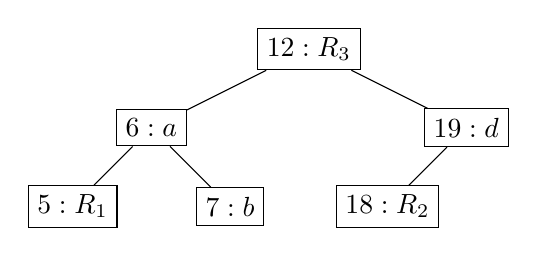
\begin{tikzpicture}
		
		\node[draw] (12) at (0,0) {$12: R_3$};
		\node[draw] (6) at (-2, -1) {$6: a$};
		\node[draw] (19) at (2, -1) {$19: d$};
		\node[draw] (18) at (1, -2) {$18: R_2$}; 
		\node[draw] (5) at (-3, -2) {$5: R_1$};
		\node[draw] (7) at (-1, -2) {$7: b$};
		
		\draw[-] (12) -- (6);
		\draw[-] (6) -- (5);
		\draw[-] (6) -- (7);
		\draw[-] (12) -- (19);
		\draw[-] (19) -- (18);
		
	\end{tikzpicture}
\end{figure}

Sei also ein Baum mit $n$ Elementen gegeben, so wie ein Intervall $[i..j]$, $i <= j$. Liegen nun $k$ Elemente, im Intervall $[i..j]$, so können alle diese Elemente insgesamt in $\mathcal{O}(k \log n)$ Laufzeit entfernt werden, da immer $\mathcal{O}(\log n)$ Laufzeit benötigt wird, um ein Element zu finden.

\subsection{Probleme}
\label{v3problems}

Die Laufzeit ist durch die beschränkte Wahl der LCP-Intervalle, \texttt{RuleIntervalIndex} und die Verbesserte Regel-Datenstruktur, erheblich verbessert, aber es gibt trotzdem noch Probleme mit V3.

\subsubsection{Speicherverbrauch}
Da V3 als erste Version auch auf Datenmengen größer als 1MB tolerable Laufzeiten erzielt, stellt sich als nächstes das Problem des Speicherverbrauchs. Allein auf einer Datenmenge von 50MB, benötigte V3 schon etwa 6-8GB oder mehr.

\subsubsection{Effizienz von RuleInvervalIndex}

Außerdem ist \texttt{RuleIntervalIndex} nicht optimal. Viele der Operationen benötigen noch mehrere Anfragen an die darunterligende Predecessor-Datenstruktur.\\
Um etwa für einen Index $i$ den Intervall-Teil des Ersetzungsintervalls zu erhalten in dem $\texttt{i}$ liegt, muss zuerst ein $\texttt{predecessor(i)}$ Aufruf durchgeführt werden, um den Intervall-Teil $\texttt{part}$zu erhalten in dem $\texttt{i}$ liegt. Dann muss eine $\texttt{get(part.totalStart)}$ Anfrage durchgeführt werden, um den ersten Intervall-Teil zu erhalten.\\
Diese Anfrage kommt oft vor, da sie benötigt wird, um zu entscheiden, ob ein Vorkommen eines Musters ersetzt werden darf.

Dazu ist das markieren, also das einfügen neuer Ersetzungsintervalle noch kostspielig. Dies benötigt ebenfalls mehrere Anfragen an die Predecessor-Struktur. Außerdem müssen für das neu einzufügende Intervall $[start, end]$ alle Intervalle mit Startpositionen im Bereich $[start, end]$ durchlaufen werden, um diese potentiell zu ersetzen, falls diese weniger tief verschachtelt sind, als das neu einzufügende Intervall. Dies kann im Worst-Case lineare Laufzeit in der Länge der Eingabe bedeuten.

\subsubsection{Zu strenge Entscheidung ob Vorkommen ersetzt werden dürfen}
\label{strictdecision}
Ein weiteres Problem ist bei der Entwicklung dieser Datenstrukturen aufgefallen. Es gibt fälle, in denen die bisher geschriebenen Algorithmen eine Ersetzung verbieten, obwohl diese eigentlich legal wäre.

Sei $p$ ein Muster mit Länge $k := |p|$. Bisher wird entschieden, ob eine Substitution von $p$ bei Index $i$ legal ist, indem geprüft wird, ob $\texttt{intervalContaining(i)}$ und $\texttt{intervalContaining(i + k - 1)}$ dieselben $\texttt{ruleId}$ und $\texttt{totalStart}$ besitzen, also die Start- und Endposition des neu entstehenden Ersetzungsintervalls in demselben Ersetzungsintervall liegen. Falls dies der Fall ist, ist eine Ersetzungs auch tatsächlich immer legal. Allerdings übersieht diese Berechung einen Fall:

Betrachten wir beispielsweise die folgende Grammatik für den String $abcdeabcd$:
\begin{align*}
	R_0 &\rightarrow R_1 c d e R_1 c d\\
	R_1 &\rightarrow a b\\
\end{align*}
Angenommen, als nächstes soll das Muster $abcd$ ersetzt werden (beachte, die Muster sind immer bezüglich des Eingabestrings, da das Suffix- und LCP array für diesen berechnet sind).
\texttt{RuleIntervalIndex} sieht hier folgendermaßen aus:
\begin{figure}[H]
	\centering
	\begin{tabular}{|c|c|c|c|} \hline
		$R_1$-$[0..1]$ & $R_0$-$[2..4]$ & $R_1$-$[5..6]$ & $R_0$-$[7..8]$ \\\hline
	\end{tabular}
\end{figure}

Das Muster $abcd$ kommt bei den Indizes $[0, 5]$ vor. Beide Ersetzungen sind offensichtlich legal, indem eine neue Regel $R_2 \rightarrow R_1cd$ eingeführt wird.\\ Versucht man aber nun mit der bisherigen Methode zu prüfen, ob die Ersetzung legal ist, so, erhält man:
\begin{align*}
	I_1 &:= \texttt{intervalContaining(0)} = R_1\text{-}[0..1]\\
	I_2 &:= \texttt{intervalContaining(0 + 4 - 1)} = R_0\text{-}[2..4]
\end{align*} 
Dabei ist dann $1 = I_1.ruleId \neq I_2.ruleId = 0$ und $0 = I_1.totalStart \neq I_2.totalStart = 2$. Die Ersetzung wird also verweigert, obwohl diese eigentlich legal wäre.\\
Diese Fälle treten ein, wenn das erste oder letzte Zeichen des zu ersetzenden Musters ein Nichtterminal ist (das Muster $abcd$ lag in der Grammatik bereits als das ersetzte $R_1 cd$ vor).

\texttt{RuleIntervalIndex} bietet zu diesem Zeitpunkt nicht die Daten um diesen Fall effizient korrekt zu entscheiden.
\newpage
% !TeX root = ../../main.tex


\tikzset{
    table nodes/.style={
        rectangle,
        draw=black,
        align=center,
        minimum height=7mm,
        text depth=0.5ex,
        text height=2ex,
        inner xsep=0pt,
        outer sep=0pt
    },      
    table/.style={
        matrix of nodes,
        row sep=-\pgflinewidth,
        column sep=-\pgflinewidth,
        nodes={
            table nodes
        },
        execute at empty cell={\node[draw=none]{};}
    }
}


\section{AreaComp V4}

Dies ist nun die finale Version dieses Algorithmus. 

\subsection{Bessere Predecessor-Datenstruktur}

Bisher verwendete \texttt{RuleIntervalIndex} Red-Black-Trees als zugrundeliegende Predecessor-Datenstruktur. Zwar ist eine Laufzeit von $\mathcal{O}(\log n)$ für jede Operation der Predecessor-Datenstruktur nicht schlecht. Da aber etwa die $\texttt{get}$ und $\texttt{predecessor}$ Operation sehr oft aufgerufen werden, stellt dies ein Bottleneck für die Laufzeit dar.
Die Idee ist nun, Red-Black-Trees durch eine für diese Zwecke effizientere Datenstruktur zu ersetzen.

Dazu bietet sich die Predecessor-Datenstruktur aus \cite{dinklage_engineering_2021} an. Im weiteren Verlauf nennen wir diese \texttt{BucketPred}. Im Code für AreaComp ist sie unter demselben Namen zu finden. Wir nutzen allerdings hier eine assoziative Variante, die durch eine Hashtabelle gestützt wird. Diese Hashtabelle ist global. 
Eine lokale Hashtabelle für jeden Bucket, scheint bei Tests keine Vorteile zu bieten.\\
Durch diese Hashtabelle erhalten wir $\mathcal{O}(1)$ amortisierte Laufzeit für $\texttt{get}$ Operationen, $\mathcal{O}(b)$ Worst-Case Laufzeit für $\texttt{predecessor}$ Operationen und $\mathcal{O}(u \backslash b)$ Laufzeit für $\texttt{insert}$ Operationen. 

Wie in \cite{dinklage_engineering_2021} beschrieben, ist es ebenfalls möglich, das hier verwendete Array von Buckets durch eine Hashtabelle zu ersetzen. Dies würde für $\texttt{insert}$ Operationen eine amortisierte $\mathcal{O}(1)$ Laufzeit bedeuten, da nun nicht mehr im Array die $\mathcal{O}(u \backslash b)$ Pointer verändert werden müssen. Allerdings würde dies auch eine Laufzeit von $\mathcal{O}(u \backslash b)$ für $\texttt{predecessor}$ Operationen bedeuten, da potenziell $\mathcal{O}(u \backslash b)$ Anfragen an die Hashtabelle gestellt werden müssen, um einen aktiven Bucket zu finden. 

Allerdings wird $\texttt{predecessor}$ viel häufiger benötigt als $\texttt{insert}$ Operationen. Daher ist es von größerer Bedeutung, dass $\texttt{predecessor}$ Aufrufe performant sind. Daher eignet sich hier das Bucket-Array besser.

Da $u = |s|$ durch den Eingabestring $s$ gegeben ist, ist also die Wahl von $b = 2^k$, für ein $k \in \mathbb{N}$, interessant. Dieser widmen wir uns bei der Evaluation.
% TODO DAS AUCH MACHEN 

\subsection{Verbesserung von \texttt{RuleIntervalIndex}}

Wie bereits beschrieben, hat die vorherige Version von \texttt{RuleIntervalIndex} das Problem, dass bestimmte Fälle, in denen eine Substitution legal ist, nicht korrekt erkannt werden. Außerdem ist das Markieren von Bereichen noch ineffizient.  

Zu diesem Zweck verändern wir die Funktionsweise von \texttt{RuleIntervalIndex} etwas.
Wir speichern nun nicht mehr die am tiefsten verschachtelten Teile von Intervallen. Stattdessen speichern wir alle existierenden Intervalle. Dies tun wir auf eine Art und Weise, die es uns trotzdem ermöglicht, effizient das tiefste verschachtelte Intervall an einem Index zu finden, aber auch gegebenfalls weniger verschachtelte Intervalle. 

\subsubsection{Beispiel}

Betrachten wir wieder die Grammatik von zuvor für den String $abcdeabcd$:
\begin{align*}
	R_0 &\rightarrow R_1 c d e R_1 c d\\
	R_1 &\rightarrow a b\\
\end{align*}
Die neue Version der Datenstruktur sieht dann folgendermaßen aus:

\begin{figure}[H]
    \centering
    \begin{tikzpicture}
        
        \matrix (A) [table, text width=7mm] {
            $a$ & $b$ & $c$ & $d$ & $e$ & $a$ & $b$ & $c$ & $d$\\
            \\
            |[draw=none]| & |[draw=none]|  &  &  &  & |[draw=none]|  & |[draw=none]|  &  & |[draw=none]|\\
            |[draw=none]| & |[draw=none]|  &  &  &  & |[draw=none]|  & |[draw=none]|  &  & |[draw=none]|\\
        };
        
        
        \node[draw, fit=(A-3-1)(A-3-9), table nodes] {$R_0$-$[0..8]$};
        \node[draw, fit=(A-4-1)(A-4-2), table nodes] {$R_1$-$[0..1]$};
        \node[draw, fit=(A-4-6)(A-4-7), table nodes] {$R_1$-$[5..6]$};
    \end{tikzpicture}
    \caption{Die neue \texttt{RuleIntervalIndex} Struktur}
    \label{newrii}
\end{figure}

\subsubsection{Neue \texttt{RuleInterval} Attribute}

Die Intervalle behalten die Attribute $\texttt{ruleId}$, $\texttt{start}$ und $\texttt{end}$ Attribute. Die anderen Attribute werden durch die Folgenden ersetzt:

\begin{itemize}[leftmargin=3cm]
    \item[\texttt{parent}] Dies ist ein Pointer auf auf das am tiefsten verschachtelte Ersetzungsintervall, das dieses Intervall enthält. Dabei muss das $\texttt{parent}$ Intervall nicht unbedingt an demselben Startindex beginnen, wie das Intervall selbst. Im obigen Beispiel zeigt der \texttt{parent} Pointer der beiden $R_1$ Intervalle auf das $R_0$ Intervall.
    \item[\texttt{firstAtStartIndex}] Ein Pointer auf das am \emph{wenigsten} verschachtelte Ersetzungsintervall, das an demselben Startindex beginnt, wie das Intervall selbst. Im Fall des Beispiels zeigen die \texttt{firstAtStartIndex} aller Intervalle jeweils auf sich selbst, da keine zwei Intervalle an demselben Index beginnen.
    \item[\texttt{nextAtStartIndex}] Ein Pointer auf das Ersetzungsintervall, das am selben Startindex beginnt und das nächst-tiefer verschachtelt ist
\end{itemize}

Die erste Idee war, in der zugrundeliegenden Predecessor-Struktur dynamische Arrays von $\texttt{RuleInterval}$s zu speichern. Dies war allerdings aufgrund des Speicherverbrauchs und des Laufzeit-Overhead von Allokationen und Reallokationen unhaltbar. Als Verbesserung sind die Elemente der Predecessor Struktur nun für jeden Index das jeweils das am tiefsten verschachtelte Intervall, das an diesem Startindex beginnt. Auf die anderen Intervalle, die an demselben Startindex beginnen, kann mithilfe der $\texttt{firstAtStartIndex}$, $\texttt{nextAtStartIndex}$ und $\texttt{parent}$ Pointer zugegriffen werden.

\subsubsection{Bestimmen der umschließenden Intervalle}
Wir können nun bestimmen, welches das tiefste verschachtelte Ersetzungsintervall ist, das ein Intervall $[i..j]$ umschließt.
Dies ist mithilfe des folgenden Algorithmus möglich.

\begin{algorithm}
    \KwIn {$from, to$ Start- und Endindizes}
    \KwOut{ $current \leftarrow floorInterval(from)$}
    \While {$current \neq \texttt{null}$} {
        \If {$current.start \leq from \textbf{ and } to \leq current.end$} {
            \KwRet{$current$}
        }
        \eIf {$current.firstAtStartIndex \leq from \textbf{ and } to \leq current.firstAtStartIndex.end$} {
            $current \leftarrow current.parent$\;
        }{
            $current \leftarrow current.firstAtStartIndex$\;
            \If {$current.parent \neq \texttt{null}$} {
                $current \leftarrow current.parent$ \;
            }
        }
    }
    \KwRet{\texttt{null}}
    \caption{intervalContaining}
\end{algorithm}

Zuerst bestimmen wir mithilfe der zugrundeliegenden Predecessor Struktur das tiefste verschachtelte Vorgänger-Intervall des Startingindex $from$. 
In der While-Schleife wird nun geprüft, ob das jetzige Intervall auch beide Grenzen einschließt. Ist dies der Fall, so haben ist dies das tiefste Intervall, das das Intervall $[from..to]$ einschießt, gefunden.\\
Ist dies nicht der Fall, so wird nacheinander entlang der $\texttt{parent}$ Pointer iteriert, bis ein Intervall gefunden wird, das beide Grenzen enthält. Da das Intervall der Startregel $R_0$ die ganze Länge des Eingabestring einnimmt, ist es also garantiert, dass solch ein Intervall auch existiert. Diese Methode kann auch das tiefste Intervall bestimmen, indem ein Index $i$ liegt, indem $\texttt{intervalContaining(i, i)}$ aufgerufen wird.

In dem Fall, dass selbst das am wenigsten verschachtelte Intervall an diesem Startindex (\texttt{firstAtStartIndex}) nicht die gegebenen Grenzen umschließt, so kann direkt zum Eltern-Intervall von \texttt{firstAtStartIndex} gesprungen werden, da somit keines der übersprungenen Intervalle die Grenzen umschließt. 

\subsubsection{Markieren von Ersetzungsintervallen}

Beim Markieren der Ersetzungsintervalle wird ein neues $\texttt{RuleInterval}$ $R_i$-$[start..end]$ in die Datenstruktur eingefügt. 
Zunächst, wird geprüft, ob es bereits ein Intervall gibt, das bei Startindex $start$ beginnt.
Hier muss zwischen verschiedenen Fällen unterschieden werden.

\begin{itemize}[leftmargin=1.5cm]
    \item[\textbf{Fall 1}] Falls kein solches Intervall existiert, so wird mithilfe von\\
    $\texttt{intervalContaining(start, end)}$ das Eltern-Intervall des neuen Intervalls bestimmt und der $\texttt{parent}$ Pointer entsprechend gesetzt.  Es wird nun nur noch das Intervall in die Predecessor Datenstruktur eingefügt.
    \item[\textbf{Fall 2}] Im Fall, dass ein solches Intervall existiert, kann es nun sein, dass das neue Intervall das nun am tiefsten verschachtelte Intervall ist, das an diesem Startindex beginnt. Ist das der Fall, so werden die Pointer des entsprechenden Index gesetzt und das neue Intervall ersetzt nun das vorherige in der Predecessor Datenstruktur, da es nun das tiefste Intervall an diesem Index ist.\\
    Ist das Intervall nicht das tiefste an diesem Index, so kann durch die $\texttt{parent}$ Pointer iteriert werden, bis ein Intervall an diesem Startindex gefunden wird, das das neue Intervall enthält. An diese Stelle muss dann das neue Intervall eingefügt werden. Es kann nun sein, das es kein solches Intervall gibt. Dann ist das neue Intervall, das größte und damit das am wenigsten verschachtelte Intervall, das an diesem Startindex beginnt. Ist das der Fall, so muss der $\texttt{firstAtStartIndex}$ aller Intervalle an diesem Startindex, auf das neue Intervall gesetzt werden. Dies kann während der ohnehin schon stattfindenden Iteration geschehen. 
\end{itemize} 

Es kann nun sein, dass durch das einfügen eines neuen Intervalls die $\texttt{parent}$ Pointer anderer Intervalle fehlerhaft werden, da sich das neue Intervall zwischen das Eltern- und
Kindintervall schieben. Dies wird nun dadurch behoben, dass über alle Intervalle der Datenstruktur, die im Intervall $[start+1..end]$ liegen, iteriert wird. In dieser Iteration wird der \texttt{parent} Pointer auf das neue Intervall gesetzt. 


\subsection{Ruleset}

Die Ruleset-Klasse ist für die Kompression des Strings verantwortlich. Das Ruleset beinhaltet eine Instanz der \texttt{RuleIntervalIndex} Datenstruktur. Sei im Folgenden $s \in \Sigma^*$ ein Eingabestring mit $n := |s|$ Dazu sind folgende Teilschritte erforderlich:

\subsubsection{Berechnen der benötigten Arrays}

Zunächst werden die benötigten Arrays berechnet. Mithilfe des QSufSort Algorithmus \cite{larsson_faster_2007} wird in $\mathcal{O}(n \log n)$ Laufzeit das Suffix-Array berechnet. Für das LCP-Array wird der Linearzeit Algorithmus aus \cite{kasai_linear-time_2001} verwendet. Zuletzt wird für die komprimierte Variante des Kind-Array der von Abouelhoda et al. beschriebene Algorithmus aus \cite{abouelhoda_optimal_2002} verwendet. Dieser berechnet das Kind-Array ebenfalls in $\mathcal{O}(n)$ Laufzeit.

\subsubsection{Berechnen der Prioritätswarteschlange}

Nun, da das Kind-Array berechnet ist, kann für jedes maximale LCP-Intervall mithilfe des von Abouelhoda et al. vorgestellten Algorithmus in $\mathcal{O}(1)$ die direkten Kind-Intervalle berechnet werden. Es existieren $\mathcal{O}(n)$ maximale LCP-Intervalle, da ein Index $i = 0,\dots,n - 1$ nicht gleichzeitig Startindex und Endindex von verschiedenen Intervallen sein kann. Insgesamt können alle maximalen LCP-Intervalle durch rekursive Aufrufe also in $\mathcal{O}(n)$ berechnet werden.

Diese Intervalle werden nun in eine auf einem Binären Heap \cite{williams_algorithm_1964} basierenden Prioritätswarteschlange eingefügt. Die benötigte Laufzeit um ein Element einzufügen oder das minimale/maximale Element zu entfernen ist $\mathcal{O}(\log n)$ im Worst-Case. Da die Aufrufe der Operationen der Prioritätswarteschlange keinen signifikanten Anteil der Laufzeit des Algorithmus ausmachen, ist es hier nicht nötig nach alternativen möglicherweise effizienteren Heap-Implementationen zu forschen.

Da die LCP-Intervalle anhand ihrer Flächenwerte priorisiert werden, muss die Flächenfunktion für jedes Intervall mindestens einmal aufgerufen werden. Sei $A$ die Flächenfunktion und $I$ ein LCP-Intervall. Sei dann die Laufzeit der Flächenfunktion $A(I)$ gleich $a(k)$, wobei $k = |I|$. 
Da die Länge jedes Intervalls $\mathcal{O}(n)$ ist, folgt insgesamt als Laufzeit für die Konstruktion der Prioritätswarteschlange: $\mathcal{O}(n \cdot a(n) \cdot \log n)$.\\\\

\subsubsection{Kompression}

Die folgenden Operationen werden solange wiederholt, bis die konstruierte Prioritätswarteschlange leer ist. 

\paragraph{Berechnung der Vorkommen}

Zuerst wird das Intervall $[i..j]$, $0 < i \leq j < n$ mit dem größten Flächenwert aus der Prioritätswarteschlange entnommen. Dann können die Indizes aller Vorkommen des Substrings in $SA[i-1..j]$ gefunden werden. Diese speichern wir in einem neuen Array $\texttt{positions}$, da diese Indizes noch nachbearbeitet werden müssen.

Die Länge des zu ersetzenden Substring $p \in \Sigma^*$ von $s$ ist dann gleich $k := |p| = \min_{i \leq a \leq j} LCP[a]$.
Dies kann in linearer Laufzeit berechnet werden, doch wir können uns hier die Eigenschaften der maximalen LCP-Intervalle und des Kind-Arrays zunutze machen. 
Wie in \cite{abouelhoda_optimal_2002} beschrieben, lässt sich der LCP-Wert eines maximalen LCP-Intervalls in $\mathcal{O}(1)$ Zeit bestimmen. Dies geschieht, indem mithilfe des $up$, beziehungsweise des $down$ Eintrages im Kind-Array, der erste $l$-Index des Intervalls bestimmt werden kann. Da an jedem $l$-Index im LCP-Array das Minimum über diesem Intervall enthält, ist damit die Länge des Substrings gefunden.

Somit sind sowohl die Vorkommen des Substrings, als auch dessen Länge berechnet. Ist $occ_p := j - i + 2$, die Anzahl an Vorkommen von $p$ in $s$. So benötigt diese Berechnung $\mathcal{O}(occ_p)$ Laufzeit, begrenzt durch die Berechnung der Indizes, an denen $p$ vorkommt.

\paragraph{Bereinigen der Indizes}

Nun ist es möglich, dass einige der Vorkommen sich nicht (mehr) für eine Ersetzung eignen. Etwa, weil diese sich mit dem vorhergehenden Vorkommen überlappen, oder weil dieses Vorkommen, die anderen nötigen Vorraussetzung für eine Substitution nicht erfüllen. Dies wurde in \ref{v3problems} und in der Beschreibung der neuen \texttt{RuleIntervalIndex} Datenstruktur genauer behandelt. Es werden nun mit den folgenden 2 Algorithmen, diejenigen Indizes entfernt, die nicht für eine Substitution in Frage kommen.

\subparagraph{substitutionAllowed}

Der erste Algorithmus bestimmt für ein Intervall, ob eine Substitution dieses Intervalls erlaubt ist. 

\begin{algorithm}
    \KwIn{$from, to: $ Start- und Endindizes, beide inklusiv,\\$intervalIndex: $ Die Instanz der \texttt{RuleIntervalIndex} Datenstruktur}
    $fromInterval \leftarrow intervalIndex.intervalContaining(from)$\;
    \While{$from = fromInterval.start \textbf{ and } to > fromInterval.end \textbf{ and }$\\$fromInterval.parent \neq \texttt{null}$} {
        $fromInterval \leftarrow fromInterval.parent$\;
    }

    \If{$to > fromInterval.end$} {
        \KwRet{$false$}
    }

    $toInterval \leftarrow intervalIndex.intervalContaining(to)$\;
    \While{$toInterval$ does not contain $fromInterval \textbf{ and }$\\$to = toInterval.end \textbf{ and } toInterval.parent \neq null$}{
        $toInterval \leftarrow toInterval.parent$\;
    }
    \KwRet{$toInterval = fromInterval$}
    
    \caption{substitutionAllowed}
\end{algorithm}
Dieser Algorithmus prüft, ob das Intervall $[from..to]$ substituiert werden darf. Dazu prüft der Algorithmus, ob sich in genau einem Ersetzungsintervall zwei Symbole (Terminale oder Nichtterminale) finden lassen, dessen vollständig expandierte Form genau bei $from$ im Eingabestring beginnt, beziehungsweise genau bei $to$ endet (inklusive des Zeichens).
In der Regel ist das Intervall das tiefste verschachtelte Intervall jeweils bei $from$ und $to$. 

Liegen $from$ oder $to$ innerhalb des tiefsten Intervalls an dem jeweiligen Index, so dürfen für den jeweiligen Index keine weniger verschachtelten Intervalle berücksichtigt werden, da sonst die Grenzen der tieferen Intervalle verletzt würden.\\ 
Fällt $from$ genau auf den Anfangsindex des tiefsten Intervalls, bei Index $from$, so kann dies ebenfalls bedeuten, dass der Index $from$ das Vorkommen eines Nichtterminals im $\texttt{parent}$ bezeichnen. Ist das der Fall, so ist es erlaubt ebenfalls die Elternintervalle mit zu berücksichtigen, solange $from$ der erste Index des jetzigen Intervalls ist. Gleiches gilt, wenn $to$ genau auf den Endindex des Intervalls fällt. Dann kann $to$ das Vorkommen eines Nichtterminals am \emph{Ende} des zu ersetzenden Bereiches in einer $\texttt{parent}$ Regel bezeichnen.

In diesen beiden Fällen gilt auch dasselbe wieder, falls $from$ auch im Elternintervall genau auf den Anfang fällt, beziehungsweise $to$ auch dort auf das Ende fällt.

Um dies besser zu veranschaulichen, hierzu ein Beispiel. Betrachten wir die folgende Grammatik für den String $abacaba$:

\begin{align*}
    S &\rightarrow AcA\\
    A &\rightarrow aba
\end{align*}

Die Methode liefert \texttt{true} für $from=0$ und $to=3$. Hier beschreibt der Index $0$ hier entweder das erste $a$ aus dem ersten Ersetzungsintervall der Regel $A$, oder das erste $A$ in der Regel $S$. Letzteres ist möglich, da der Index $0$ genau auf den Anfang des Ersetzungsintervalls $[0..2]$ der Regel $A$ fällt. Der Index $3$ kann hier nur $c$ beschreiben.
Es lassen sich hier also das erste $A$ als Startsymbol, und das $c$ als Endsymbol finden, die beide in dem einen Ersetzungsintervall der Regel $S$ liegen. Damit ist die Ersetzung von $Ac$ in der Regel $S$ erlaubt.

Für $from=1$ und $to=3$ liefert die Methode allerdings \texttt{false}. Der Index $3$ liefert wie im vorhergehenden Fall wieder nur das $c$ aus Regel $S$.
Index $1$ allerdings, liefert nur das $b$ aus dem ersten Ersetzungsintervall der Regel $A$. Hier dürfen keine weniger tiefen Ersetzungsintervalle (in diesem Fall nur das Eine der Regel $S$) berücksichtigt werden, da der Index $1$ nicht der Anfangsindex des Ersetzungsintervalls ist, in dem dieser Index liegt.
Wir haben als Wahl für das Startsymbol nur $b$ aus Regel $A$ und als Endsymbol nur das $c$ aus Regel $S$. Hier lassen sich also kein Paar von Start- und Endsymbolen finden, die in demselben Ersetzungsintervall liegen. Die Substitution ist als ungültig.

Für $from=0$ und $to=5$ liefert die Methode ebenfalls \texttt{false}. Hier liefert der Index $0$ wie im ersten Fall wieder $a$ aus dem ersten Ersetzungsintervall der Regel $A$ und das erste $A$ in der Regel $S$. Index $5$ liefert hier nur das $b$ aus dem \emph{zweiten} Ersetzungsintervall der Regel $A$. 
Da wir als Wahl für das Endsymbol nur das $b$ aus einem Ersetzungsintervall der Regel $A$ zur Verfügung haben, kommt für das Startsymbol nur das $a$ infrage, da das $A$ aus einem Ersetzungsintervall der Regel $S$ stammt.
Allerdings ist die Kombination von $a$ als Startsymbol und $b$ als Endsymbol ebenfalls ungültig, da diese jeweils aus unterschiedlichen Ersetzungsintervallen stammen.
Die Substitution ist hier also auch ungültig.

\subparagraph{cleanPositions}

Mithilfe des vorherigen Algorithmus lassen sich nun die gegebenen Indizes der Vorkommen von $p$ bereinigen, sodass nur noch Indizes übrig bleiben, bei denen es auch tatsächlich möglich ist, das Vorkommen zu ersetzen. Der folgende Algorithmus leistet dies, und gibt zusätzlich die Anzahl der übrigen Positionen zurück. In diesem Algorithmus werden Positionen entfernt, indem sie durch $-1$ ersetzt werden. Beachte, dass dieser Algorithmus erwartet, dass das $positions$ Array aufsteigend sortiert ist.

\begin{algorithm}
    \KwIn{ $positions: $ Array von Indizes an denen $p$ vorkommt, $len: $ Länge von $p$}
    $count \leftarrow 0$\;
    $previous \leftarrow -\infty$\;
    \For{$i$ \textbf{in} $0$ \textbf{to} $n - 1$} {
        $pos \leftarrow positions[i]$\;
        \eIf{$previous + len \leq pos$ \textbf{ and } $substitutionAllowed(pos, pos + len - 1)$}{
            $previous \leftarrow pos$\;
            $count \leftarrow count + 1$\;
        }{
            $positions[i] \leftarrow -1$\;
        }
    }
    \KwRet{$count$}
    \caption{cleanPositions}
\end{algorithm}

Der Algorithmus iteriert durch das Array der gegebenen Positionen. Falls dann das jetzige Vorkommen sich nicht mit dem Vorherigen überschneidet und eine Substitution dieses Vorkommens erlaubt ist, so erhöhe den Zähler. Falls dies nicht der Fall ist, so entferne dieses Vorkommen.

\paragraph{Sicherstellen unterschiedlicher Vorkommen}

Es stellt sich nun ein weiteres Problem. Da das Suffix- und LCP-Array global für den Eingabestring berechnet werden, ist es möglich, dass es zwar mehrere Vorkommen eines Musters im Eingabestring gibt, aber durch vorhergehende Substitutionen dieses Vorkommen nur noch einmal in der Grammatik vorkommt. Betrachten wir wieder das Beispiel von vorher:

\begin{align*}
    S &\rightarrow AcA\\
    A &\rightarrow aba
\end{align*}

Angenommen, das zu ersetzende Muster sei $ab$ an den Positionen $[0, 4]$. Dies sind zwei unterschiedliche nicht-überlappende Vorkommen im Eingabestring, die auch theoretisch ersetzt werden dürften. Allerdings sehen wir in der Grammatik, dass diese beiden Vorkommen nur zusammengefasst in der rechten Seite der Regel $A$ vorkommen. Insgesamt kommt $ab$ also nur ein einziges Mal in der Grammatik vor. Es müssen also verschiedene Vorkommen \emph{in der Grammatik} existieren, damit eine Substitution überhaupt eine Kompression ermöglicht.

Dies leistet der folgende Algorithmus. Er liefert \texttt{true}, falls es mehrere tatsächlich unterschiedliche Vorkommen gibt, solst \texttt{false}:

\begin{algorithm}
    \KwIn{ $positions: $ Array von Indizes an denen $p$ vorkommt, entfernte Positionen $=-1$}
    $set \leftarrow \emptyset$\;
    $firstRuleId = -1$\;
    \For{$pos$ \textbf{in} $positions$} {
        \If{$pos == -1$} { 
            \textbf{continue}\;
        }
        $ruleInterval \leftarrow intervalIndex.intervalContaining(pos)$\;
        $ruleId \leftarrow ruleInterval.ruleId$\;
        $startIndex \leftarrow ruleInterval.start$\;

        \If{$firstRuleId = -1$} {
            $firstRuleId \leftarrow ruleId$\;
        }
        \ElseIf{$ruleId \neq firstRuleId$ \textbf{ or } $startIndex \in set$} {
            \KwRet{$true$}
        }
        $set \leftarrow set \cup \{startIndex\}$\;
    }
    \KwRet{$false$}
    
    \caption{differingOccurrences}
\end{algorithm}

Der Algorithmus verwaltet eine zunächst leere Menge, die die Startindizes derjenigen Ersetzungsintervalle, in denen bereits ein Vorkommen des Musters gefunden wurde. Hierbei werden nur jeweils die tiefsten Intervalle berücksichtigt. Außerdem speichert der Algorithmus die ID der ersten Regel, die in der nun folgenden for-Schleife gefunden wird.

Die for-Schleife iteriert durch die vom vorherigen Schritt noch übrigen Positionen und berechnet jeweils das tiefste Intervall an dem gegebenen Index, sowie dessen ID und Startindex. Ist die $firstRuleId$ noch nicht gesetzt, so wird diese auf die ID des berechneten Intervalls gesetzt. Andernfalls wird geprüft, ob die ID des soeben berechneten Intervalls mit der als erstes berechneten Intervalls übereinstimmt. Stimmen diese nicht überein, so sind bereits zwei Vorkommen in unterschiedlichen Regeln gefunden worden. Diese müssen zwangsweise unterschiedlich sein. Also gibt der Algorithmus dann \texttt{true} zurück.

Ist dies nicht der Fall, so wird geprüft ob der Startindex des jetzigen Intervalls bereits in der Menge zu finden ist, also schon ein Vorkommen in einem Intervall mit diesem Startindex gefunden wurde. Wenn ja, dann muss das aktuell betrachtete Vorkommen zwangsweise unterschiedlich mit dem bereits gefundenen sein. Denn es gibt hier zwei Fälle:
\begin{itemize}
    \item[\textbf{Fall 1}] \emph{Das jetzige Intervall ist dasselbe Intervall, indem bereits ein Vorkommen gefunden wurde.}\\
    In diesem Fall existiert also in demselben Intervall ein Vorkommen an einem kleineren Index. Dies gilt, da die Indizes aufsteigend sortiert sind (ausgenommen der entfernten Indizes) und an jedem Index nur maximal \emph{ein} Intervall mit einer gegebenen Regel ID existieren kann. 
    \item[\textbf{Fall 2}] \emph{Das jetzige Intervall ist ein anderes Intervall, das an demselben Startindex beginnt.}\\
    Wie in Fall 1 schon beschrieben, muss also das jetzige Intervall einer anderen Regel angehlören. Da nun ein Vorkommen in einer anderen Regel gefunden wurde, als das vorherige Vorkommen, so folgt sofort, dass das jetzige Vorkommen unterschiedlich sein muss. 
\end{itemize}   
Also wird \texttt{true} zurückgegeben, wenn ein Startindex zweimal gefunden wird.

Tritt keine dieser Bedingungen je ein, so existieren keine unterschiedlichen Vorkommen und der Algorithmus gibt $\texttt{false}$ zurück.\\\\
Gibt dieser Algorithmus \texttt{false} zurück, so wird keine Substitution durchgeführt, da insgesamt nur ein Vorkommen des Musters in der Grammatik existiert.

\newpage
\paragraph{Faktorisierung}

Der letzte Schritt der Kompression ist die tatsächliche Substitution der Vorkommen des Musters.
\begin{algorithm}
        \KwIn{ $len: $ Länge des Musters,\\ $positions: $ Array mit Startindizes der Vorkommen. Entfernte Vorkommen sind $-1$,\\ $intervalIndex: $ Die Instanz der \texttt{RuleIntervalIndex} Datenstruktur}
        $nextId \leftarrow$ nächste unbenutzte Regel ID\;
        \For{$pos \leftarrow positions$} {
            \If{$pos = -1$} {
                \textbf{continue}\;
            }
            $intervalIndex.mark(nextId, pos, pos + len - 1)$\;
        }
\end{algorithm}

Der Algorithmus iteriert nur durch das Array der Startindizes der Vorkommen des Musters und markiert die jeweiligen Intervalle, die das Vorkommen des Musters einnimmt, in der Datenstruktur. 

\paragraph{Abschluss des Algorithmus}

Wenn der Algorithmus terminiert, so sind alle Ersetzungsintervalle in der \texttt{RuleIntervalIndex} Datenstruktur gespeichert.
Diese lässt sich mithilfe des Eingabestrings die Grammatik in eine Darstellung überführen, in der die Produktionsregeln der Grammatik explizit gespeichert werden.
Es kann für jedes Zeichen im Eingabestring die tiefste Regel bestimmt werden, in der das jeweilige Zeichen liegt, und in eine entsprechende Liste von Zeichen eingefügt werden.

Hierzu werden 2 Stacks angewendet.
\begin{itemize}[leftmargin=2cm]
    \item[\texttt{nestingStack}] Ein Stack von Ersetzungsintervallen. Ist die Iteration bei Index $i$, so enthält \texttt{nestingStack} alle Ersetzungsintervalle in denen $i$ liegt, in der Reihenfolge ihrer Verschachtelung. Dabei liegt das am tiefsten verschachtelte Intervall oben auf dem Stack.
    \item[\texttt{symbolStack}] Ein Stack von Listen von Symbolen. Für jedes Ersetzungsintervall enthält \texttt{symbolStack} jeweils eine korrespondierende Liste von Symbolen. 
    Ist die Iteration bei Index $i$, so enthalten die Listen jeweils Symbole der rechten Seite der Produktionsregel, die durch das korrespondierende Ersetzungsintervall repräsentiert wird. Sie enthalten Symbole, die in dem Ersetzungsintervall bis zum Index $i$ im Eingabestring vorkommen. 
\end{itemize} 

Ein Beispiel dafür. Betrachten wir die folgende Grammatik für $abcdabeabcd$

\begin{align*}
    S &\rightarrow ABeA\\
    A &\rightarrow Bcd\\
    B &\rightarrow ab\\
\end{align*}

\begin{figure}[H]
    \centering
    \begin{tikzpicture}
        \matrix (A) [table, text width=7mm] {
            $a$ & $b$ & $c$ & $d$ & $a$ & $b$ & $e$ & $a$ & $b$ & $c$ & $d$\\
            \\
            |[draw=none]| & |[draw=none]|  &  &  &  &  &  & |[draw=none]|  & |[draw=none]|  &  & |[draw=none]|\\
            |[draw=none]| & |[draw=none]|  &  &  &  &  &  & |[draw=none]|  & |[draw=none]|  &  & |[draw=none]|\\
        };
        
        \node[draw, fit=(A-3-1)(A-3-9), table nodes] {$R_0$-$[0..10]$};

    \end{tikzpicture}
\end{figure}

